\section[Nine patch]{.9.png文件}
在使用"draw9patch"工具绘制.9.png图片文件时,图片的四个边各有不同的含义,
对比图\ref{fig:draw9patch}可以更加直观的理解,
\begin{figure}
  \centering
  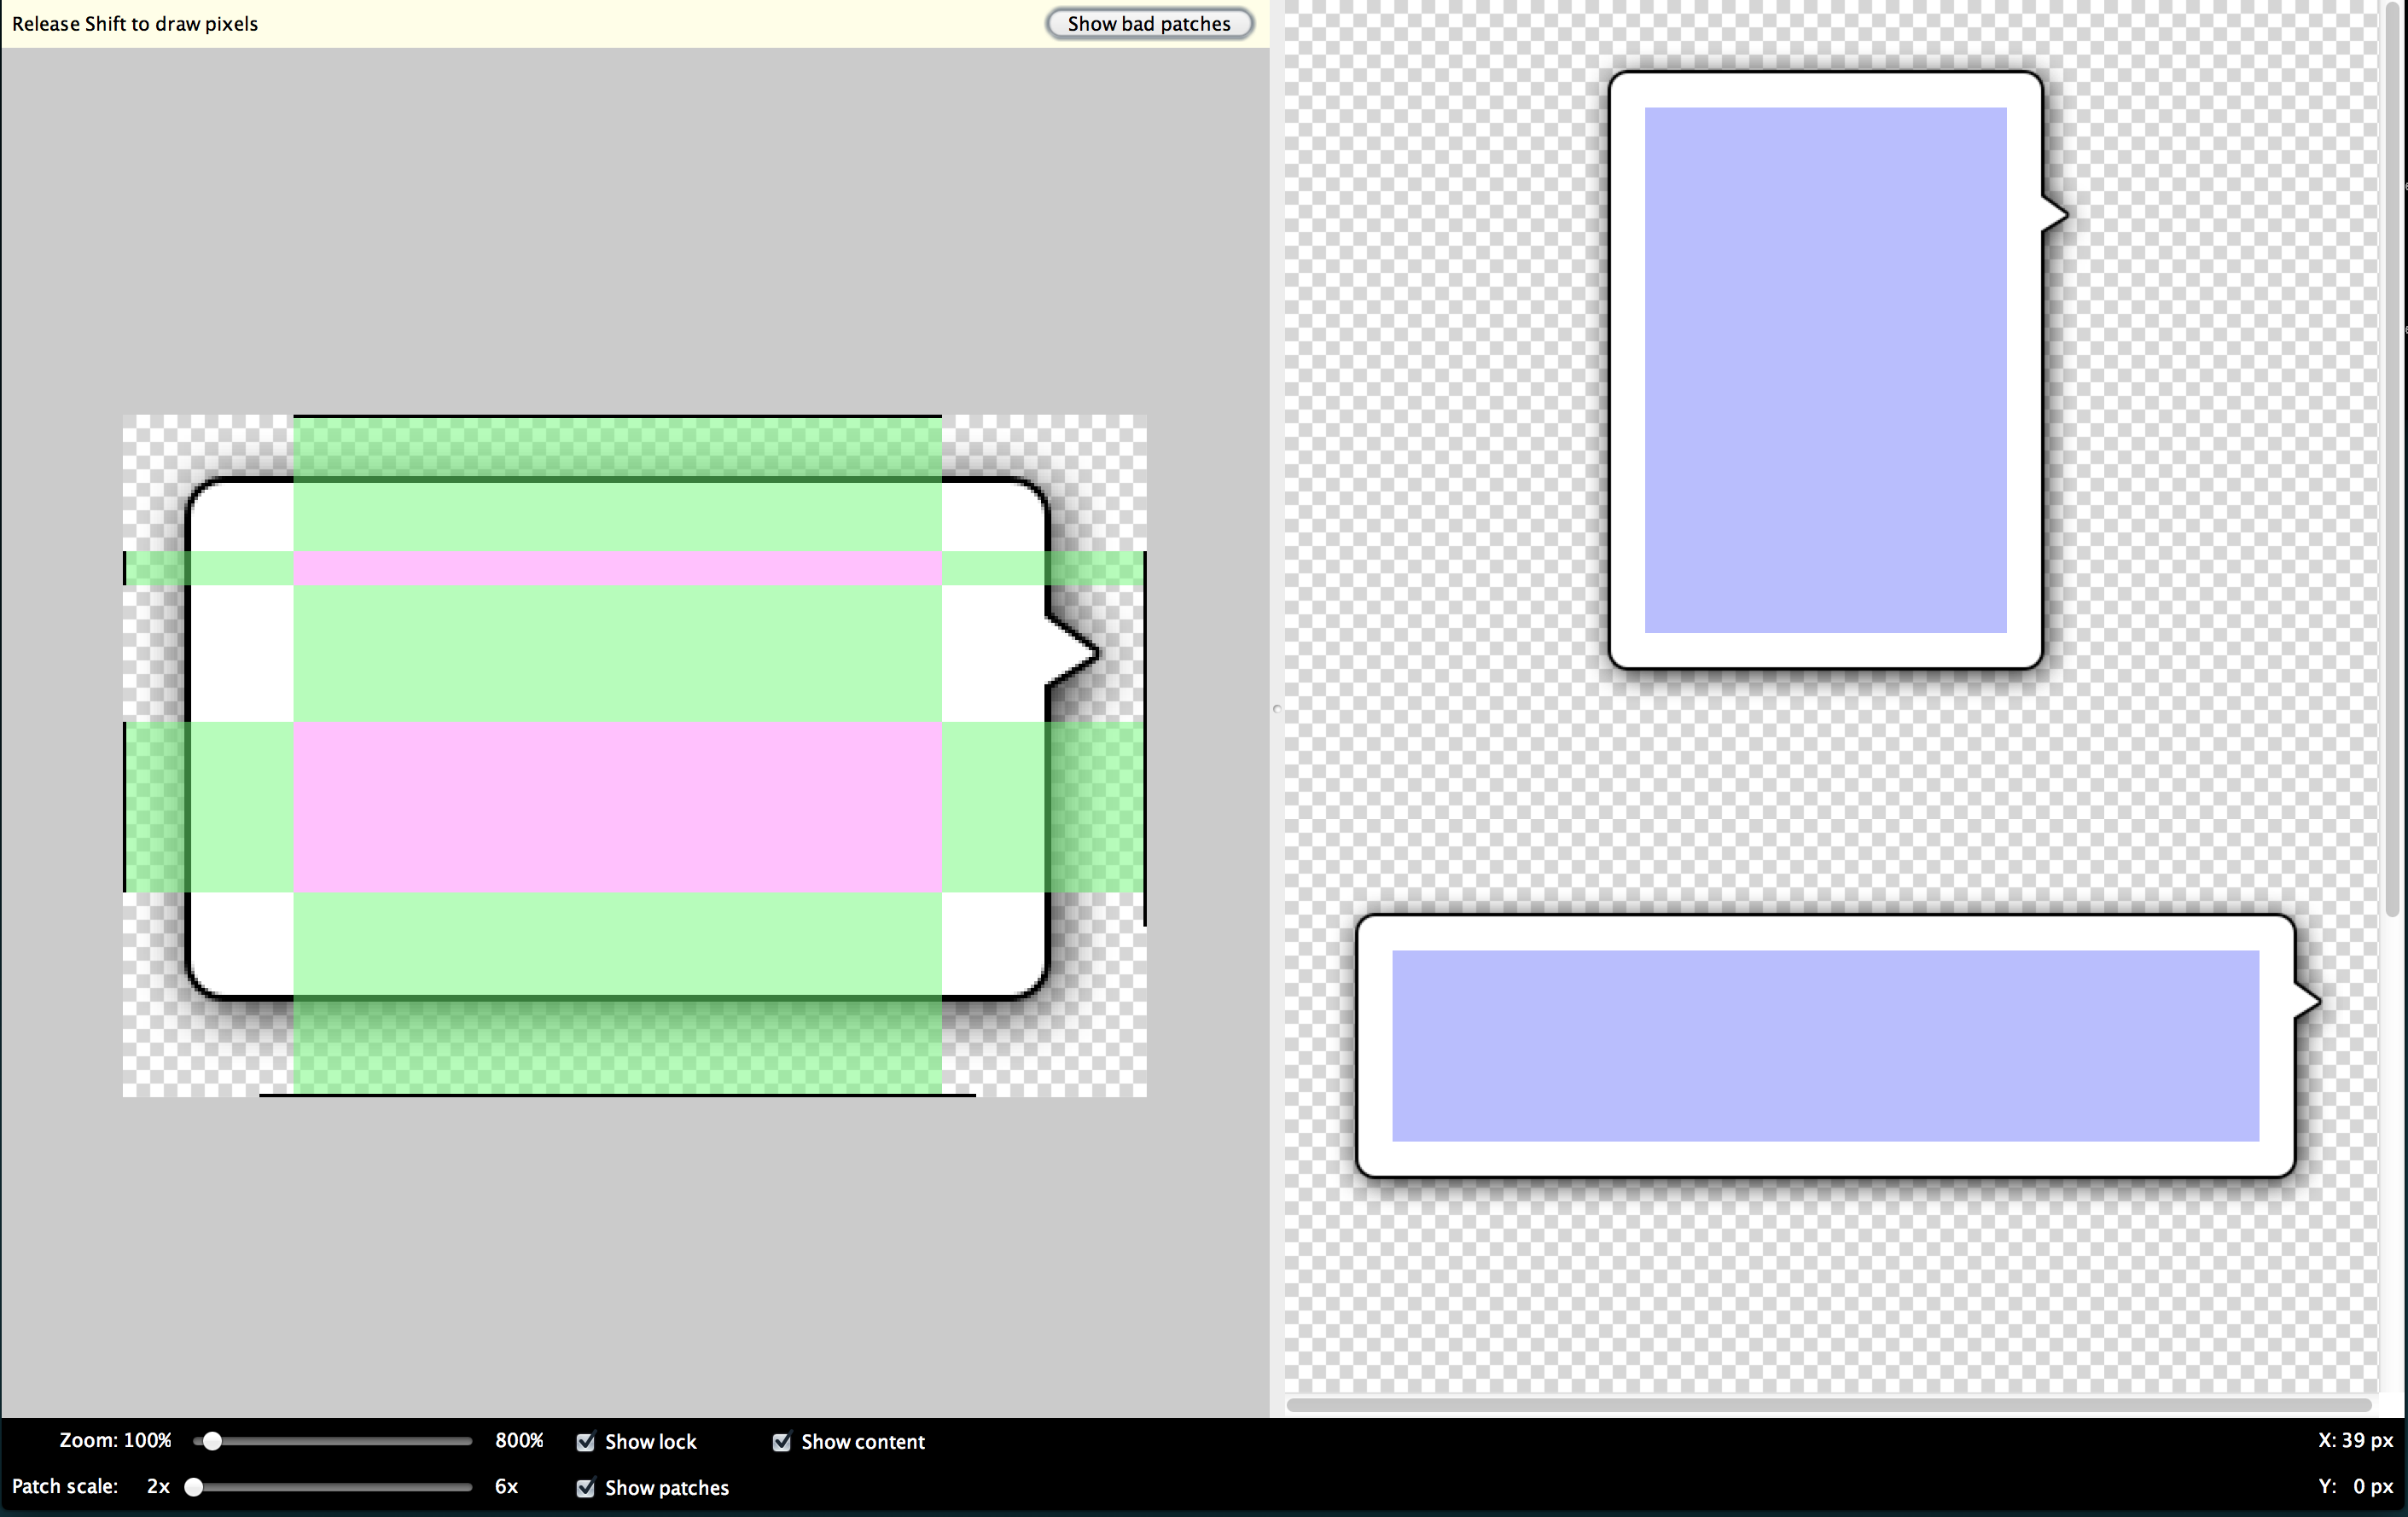
\includegraphics[width=.8\textwidth]{picturedir/draw9patch.png}\\
  \caption{9 patch file in Android}\label{fig:draw9patch}
\end{figure}

\begin{description}
  \item[vertical stretching: ] left side上的黑色部分
  \item[horizontal stretching: ] top side上的黑色部分
  \item[vertical content: ] right size上的黑色部分
  \item[horizontal content: ] bottom side上的黑色部分
\end{description}
stretching area表示可以自由缩放的部分,content area表示当.9.png作为View
的背景时,View的content部分,比如TextView的文字部分。

bounds(轮廓)以内、content之外的部分,将被设置为View的“默认”padding,这个
需要特别注意,有时在使用.9.png作为背景之后,View莫名其妙的增加了padding,
很有可能就是这个“默认”padding导致的!解决方法其实很简单,手动设置View的
padding值即可。当然,更加规范的做法是在生成.9.png文件时,分别设置四个边
上的内容,这样用默认的padding生成的View更美观,手动设置View的padding有可能
使得内容与背景不吻合,毕竟作图的人比写代码的人更加了解图片。